\documentclass[a4paper,11pt,fleqn]{article}%fleqn pour aligner les equations à gauche
\usepackage{../../Styles/Cours}


\newcommand{\chnum}{Chapitre 12}
\newcommand{\chtitle}{Accélérateur de particules}
\newcommand{\dtype}{TP}


  \begin{document}

  \maketitle
  
Les accélérateurs de particules sont utilisés dans différents domaines, notamment le domaine médical, mais également en physique subatomique pour étudier la composition des particules. \textbf{Comment peut-on augmenter l'énergie cinétique d'une particule chargée ?}
\noindent
\begin{figure}[h!]
\begin{minipage}{.38\linewidth}
\begin{tcolorbox}[arc=1ex, colframe=black, left=3pt, right=3pt, top=3pt, bottom=2pt, height=7.5cm]
\caption*{\textbf{Document 1 : Créaction d'un champ électrique}}
\centering
\begin{circuitikz}[scale=1.2, transform shape]
\draw (0,0)
	to[V] (3.5,0)
	to[short] (3.5,0)
	to[short] (3.5,-2)
	to (2.5,-2);
\draw[thick] (2.5,-1.5)--(2.5,-2.5);
\node[below] (B) at (2.5,-2.5){\textbf{B}};
\draw[thick] (1,-1.5)--(1,-2.5);
\node[below] (A) at (1,-2.5){\textbf{A}};
\draw (0,0)
	to[short] (0,-2)
	to (1,-2);
\draw (1,-1.5) 
  to[open, v>=$\vec{E}$,red] (2.5,-1.5);
\end{circuitikz}
\end{tcolorbox}
\end{minipage}\hspace{.02\linewidth}
\begin{minipage}{.6\linewidth}
	\begin{tcolorbox}[arc=1ex, colframe=black, left=3pt, right=3pt, top=3pt, bottom=2pt, height=7.5cm]
\caption*{\textbf{Document 2 : Travail de la force}}
Une particule de charge $q$ dans un champ électrique $\vec{E}$ subit une force électrique $\vec{F_e}$ égale à :
\begin{eqnarray}
	\vec{F_e}=q \cdot \vec{E} \nonumber
\end{eqnarray}
Le travail de la force électrique $W_{AB}(\vec{F_e})$, exprimé en joule ($J$), correspond à :
$$W_{AB}(\vec{F_e})= \vec{F_e} \cdot \vec{AB} = q \cdot U_{AB} $$

\begin{itemize**}
	\item $AB$ : distance entre les plaques ($m$ )
	\item $q$ : charge électrique de la particule ($C$)
	\item $U_{AB}$ : tension entre les plaques ($V$ )
\end{itemize**}
\end{tcolorbox}
\end{minipage}
\begin{minipage}{.58\linewidth}
\begin{tcolorbox}[arc=1ex, colframe=black, left=3pt, right=3pt, top=3pt, bottom=2pt, height=9.2cm]
\caption*{\textbf{Document 3 : Principe d'un accélérateur linéaire}}
Un accélérateur linéaire de particules est un appareil permettant de communiquer de l'énergie cinétique à une particule chargée.\\
En 1928, Rolf Wider\o e fut l'un des premiers à construire un tel accélérateur, afin de communiquer à des ions potassium \ce{K+} une énergie cinétique de \SI{50}{\electronvolt}. Son accélérateur était constitué d'une source $S$ et d'une succession de tubes sous vide séparés par des interstices.\\
Les sections de deux cylindres adjacents présentent des charges de signes opposés : un champ électrique $\vec{E}$ règne donc dans ces interstices. À l'intérieur des tubes, le champ électrique est nul, les particules s'y déplacent à vitesse constante.\\
La tension du générateur étant alternative, les sections des cylindres voient le signe de leur charge changer après chaque passage de particule. 
\end{tcolorbox}
\end{minipage}\hspace{.02\linewidth}
\begin{minipage}{.4\linewidth}
\begin{tcolorbox}[arc=1ex, colframe=black, left=3pt, right=3pt, top=3pt, bottom=2pt, height=9.2cm]
\caption*{\textbf{Document 4 : Schéma de Linac de Wider\o e}}
Le schéma ci-dessous décrit l'un des deux états possibles de l'accélérateur, pour une particule se trouvant entre la source, chargée positivement, et le premier tube, chargé négativement.\\
\begin{center}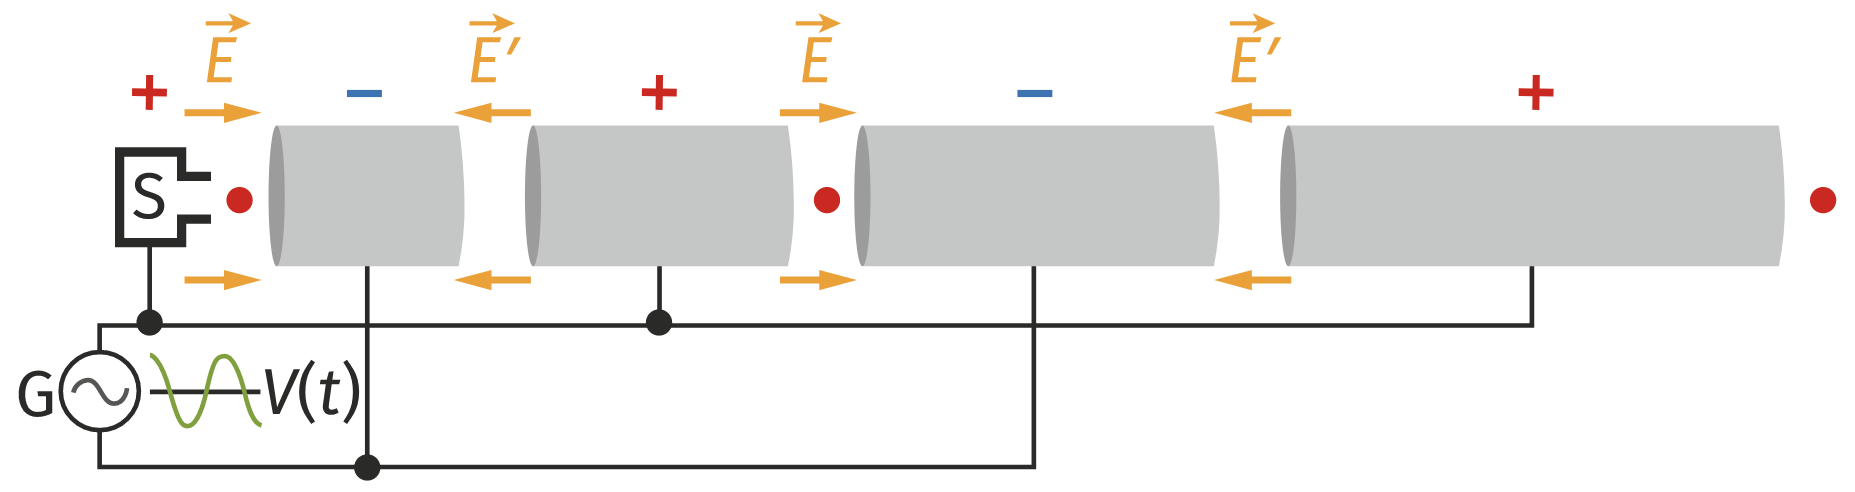
\includegraphics[scale=.11]{Ressources/TSPE_C5_Act2_Fig2.png}\end{center}
\end{tcolorbox}
\end{minipage}
\end{figure}
\\ \textbf{Données :}
\begin{itemize*}
	\item Masse d'un ion potassium $K^{+}$ : $m$ = \SI{6,5E-26}{\kilo \gram}
	\item Conversion d'unité : \SI{1}{eV} = \SI{1,60E-19}{\joule}
\end{itemize*}
\begin{enumerate}
	\item En utilisant le théorème de l'énergie cinétique, expliquer à quelle condition une particule de charge $q$ peut être accéléré par un champ électrique $\vec{E}$.
	\item Selon le \textbf{Document 3}, déterminer la vitesse $v_{finale}$ d'un ion potassium \ce{K+} à la sortie de l'accélérateur.
	\item Reproduire le schéma du \textbf{Document 4} et faire les modifications nécessaires pour qu'il corresponde à l'autre alternance de la tension. Justifier cette alternance.
	\item \textbf{Synthèse : } Décrire le fonctionnement d'un accélérateur linéaire de particule.
\end{enumerate}
\end{document}